\documentclass[a4paper,10pt]{article}
\usepackage[utf8]{inputenc}
\usepackage{amsmath}
\usepackage{fullpage}
\usepackage{hyperref}
\usepackage{cleveref}
\usepackage{graphicx}
\usepackage{listings}
\usepackage{color}
\usepackage{float}
\usepackage{apacite}

\definecolor{mygreen}{rgb}{0,0.6,0}
\definecolor{mygray}{rgb}{0.5,0.5,0.5}
\definecolor{mymauve}{rgb}{0.58,0,0.82}

\lstset{ 
  backgroundcolor=\color{white},   % choose the background color; you must add \usepackage{color} or \usepackage{xcolor}; should come as last argument
  basicstyle=\footnotesize,        % the size of the fonts that are used for the code
  breakatwhitespace=false,         % sets if automatic breaks should only happen at whitespace
  breaklines=true,                 % sets automatic line breaking
  captionpos=b,                    % sets the caption-position to bottom
  commentstyle=\color{mygreen},    % comment style
  deletekeywords={...},            % if you want to delete keywords from the given language
  escapeinside={\%*}{*)},          % if you want to add LaTeX within your code
  extendedchars=true,              % lets you use non-ASCII characters; for 8-bits encodings only, does not work with UTF-8
  firstnumber=1,                   % start line enumeration with line 1000
  frame=single,	                   % adds a frame around the code
  keepspaces=true,                 % keeps spaces in text, useful for keeping indentation of code (possibly needs columns=flexible)
  keywordstyle=\color{blue},       % keyword style
  language=Python,                 % the language of the code
  morekeywords={*,...},            % if you want to add more keywords to the set
  numbers=left,                    % where to put the line-numbers; possible values are (none, left, right)
  numbersep=5pt,                   % how far the line-numbers are from the code
  numberstyle=\tiny\color{mygray}, % the style that is used for the line-numbers
  rulecolor=\color{black},         % if not set, the frame-color may be changed on line-breaks within not-black text (e.g. comments (green here))
  showspaces=false,                % show spaces everywhere adding particular underscores; it overrides 'showstringspaces'
  showstringspaces=false,          % underline spaces within strings only
  showtabs=false,                  % show tabs within strings adding particular underscores
  stepnumber=1,                    % the step between two line-numbers. If it's 1, each line will be numbered
  stringstyle=\color{mymauve},     % string literal style
  tabsize=4,	                   % sets default tabsize to 2 spaces
  title=\lstname                   % show the filename of files included with \lstinputlisting; also try caption instead of title
}


%opening
\title{Handin Assignment 2}
\author{Ioannis Koutalios s3365530}

\begin{document}

\maketitle

\begin{abstract}
 Code and results for Handin assignment 2 for the course Numerical Recipes in Astrophysics.
\end{abstract}

\section{Satellite galaxies around a massive central}

For satellite galaxies from near the centre up to 5 virial radii, we can assume a density profile that follows the equation

\begin{equation}
  n(x) = A \langle N_{sat} \rangle \left(\frac{x}{b}\right)^{a-3} \exp[-\left(\frac{x}{b}\right)^c]
\end{equation}
where x is the radius relative to the virial radius($x=r/r_{vir}$) and $a,\, b,\, c$ are free parameters which for our purposes we assume to be $a=2.4,\, b = 0.25,\, c = 1.6$. $\langle N_{sat} \rangle $ is the average total number of satellites, which for this exercise is 100, and $A$ is a normalization factor. 

\subsection{Numerical Integration}

We want to calculate $A$. To do that we need to solve 
\begin{equation}
  \iiint_V n(x) dV = \langle N_{sat} \rangle 
\end{equation}

which can be written as 

\begin{equation}
  \int_{\phi=0}^{2\pi} \int_{\theta=0}^{\pi} \int_{x=0}^{5} n(x) x^2 \sin(\theta) d\phi d\theta dx = 4 \pi \int_{x=0}^{5} n(x) x^2 dx = \langle N_{sat} \rangle 
\end{equation}

We want to numerically solve the final integral. To do that we define our function ``f\_n'' which is equivalent to $4 \pi n(x) x^2$. We then define the ``trapezoid'' function which uses the trapezoid rule to calculate the integral. We can directly integrate using this function but we will be more accurate if we integrate using Romberg's algorithm. The function ``romberg'' applies this algorithm. It initializes an array of integrals by calling the ``trapezoid'' function for an increasing number of points and then uses Richardson's extrapolation to combine these estimates and return a final value. The order of the extrapolation is $m$ and can be specified when calling the function.    

\lstinputlisting{open_int.py}

In the main part of the script, we calculate the integral using Romberg's algorithm for an initial number of points $n=10\,000$ and an extrapolation order of $m=5$. We then calculate $A$ by dividing 100 by the value we calculated and print A using 10 significant digits. The output of the script can be seen below. 

\lstinputlisting{output/open_int.txt}


\subsection{Distribution}

For the next task, we have to sample galaxies using the distribution. The probability distribution of the relative radii should be $p(x) dx = N(x) dx / \langle N_{sat} \rangle$, where $N(x)$ is:
\begin{equation}
  N(x)= \int_{\phi=0}^{2\pi} \int_{\theta=0}^{\pi} n(x) x^2 \sin(\theta) d\phi d\theta =4 \pi n(x) x^2
\end{equation}

We also want to uniformly sample the angle $\phi,\,\theta$ in their respective range. 

To do that we first import from our previous script the function ``n'' with the defined parameters. We also read the calculated value of $A$ from the output of our previous script. We then define ``f\_N'' to be our $N(x)$ function from above. 

We create a function ``lcg'' for generating random numbers using the algorithm for a Linear Congruential Generator. We normalize the numbers we return so they are uniformly distributed between 0 and 1. The values we selected for the multiplier, increment and modulus come from previous implementations of the same algorithm in many scientific libraries. The ``uniform'' function utilizes the ``lcg'' to uniformly generate values in any given range. 

Our next function ``sampling'' uses rejection sampling to generate values for a given distribution. We use two seeds one for the numbers we generate and one for the testing values to perform the rejection process. We want to sample N values so we generate more to account for the rejection process. The final array of generated values is of length N.

\lstinputlisting{distr.py}

In the main part of our script, we generate our sampled galaxies. We create an array which has a shape of ($3 \times 10\,000$) to store for each galaxy the relative radius, and the two angles. We then store it for the next task and create the histogram plots. Along with the histogram plots, we also plot $N(x)/100$. The correction of $N(x)$ is to account for the normalization offset of $10\,000/\langle N_{sat} \rangle = 100$

As we can see in \Cref{fig:distr} there is a great match between the normalized distribution and our sample of generated galaxies. On the right panel, we can see that the line crosses every bin at its top, as we would expect.  


\begin{figure}[H]
  \centering
  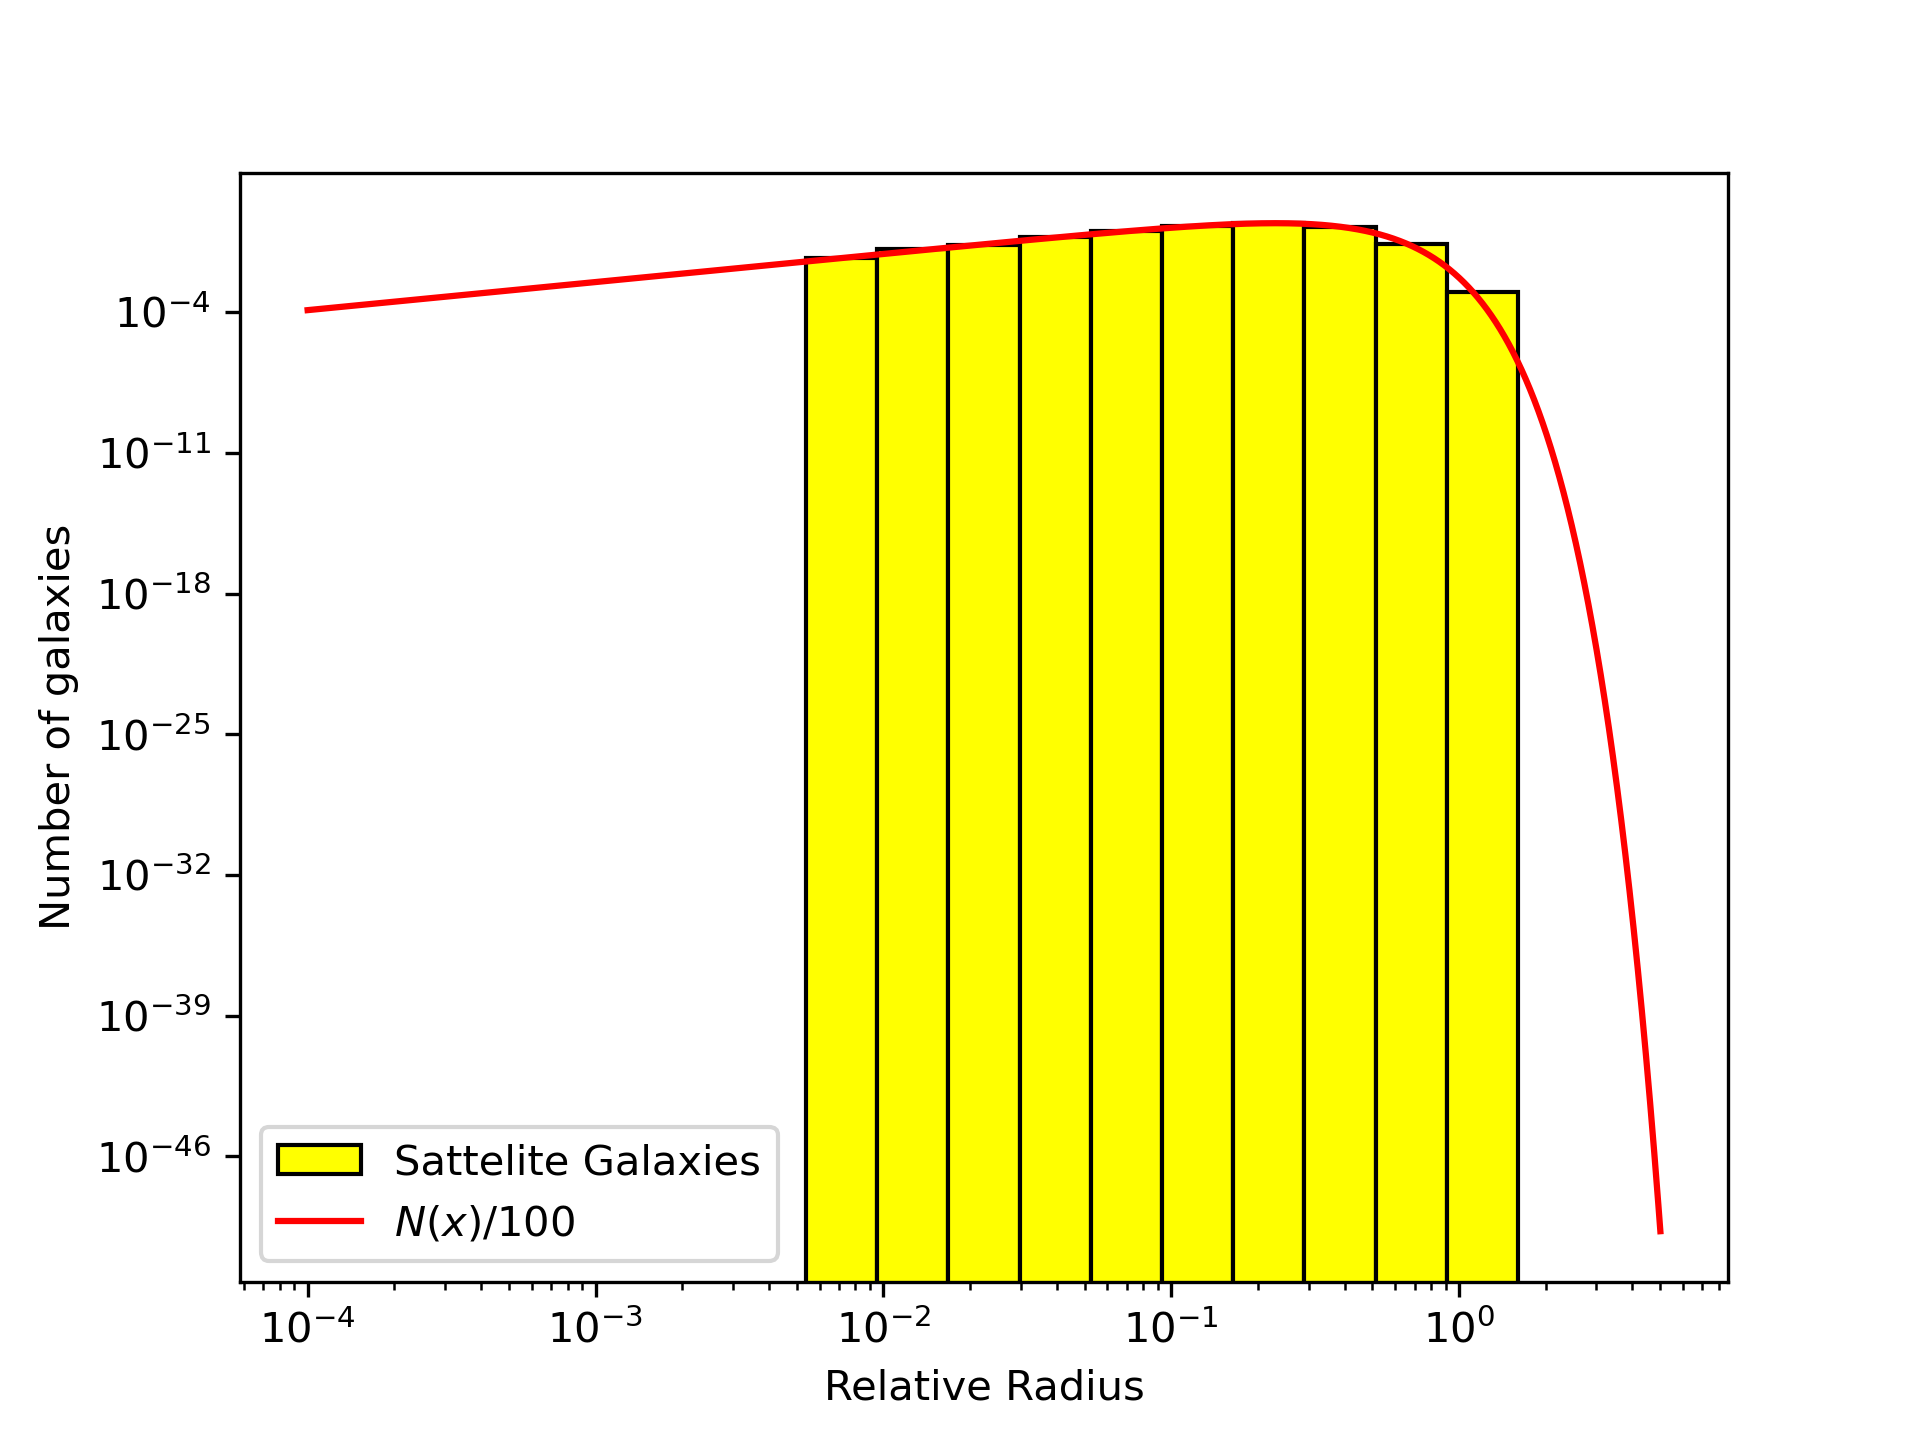
\includegraphics[width=0.49\linewidth]{./plots/distr.png}
  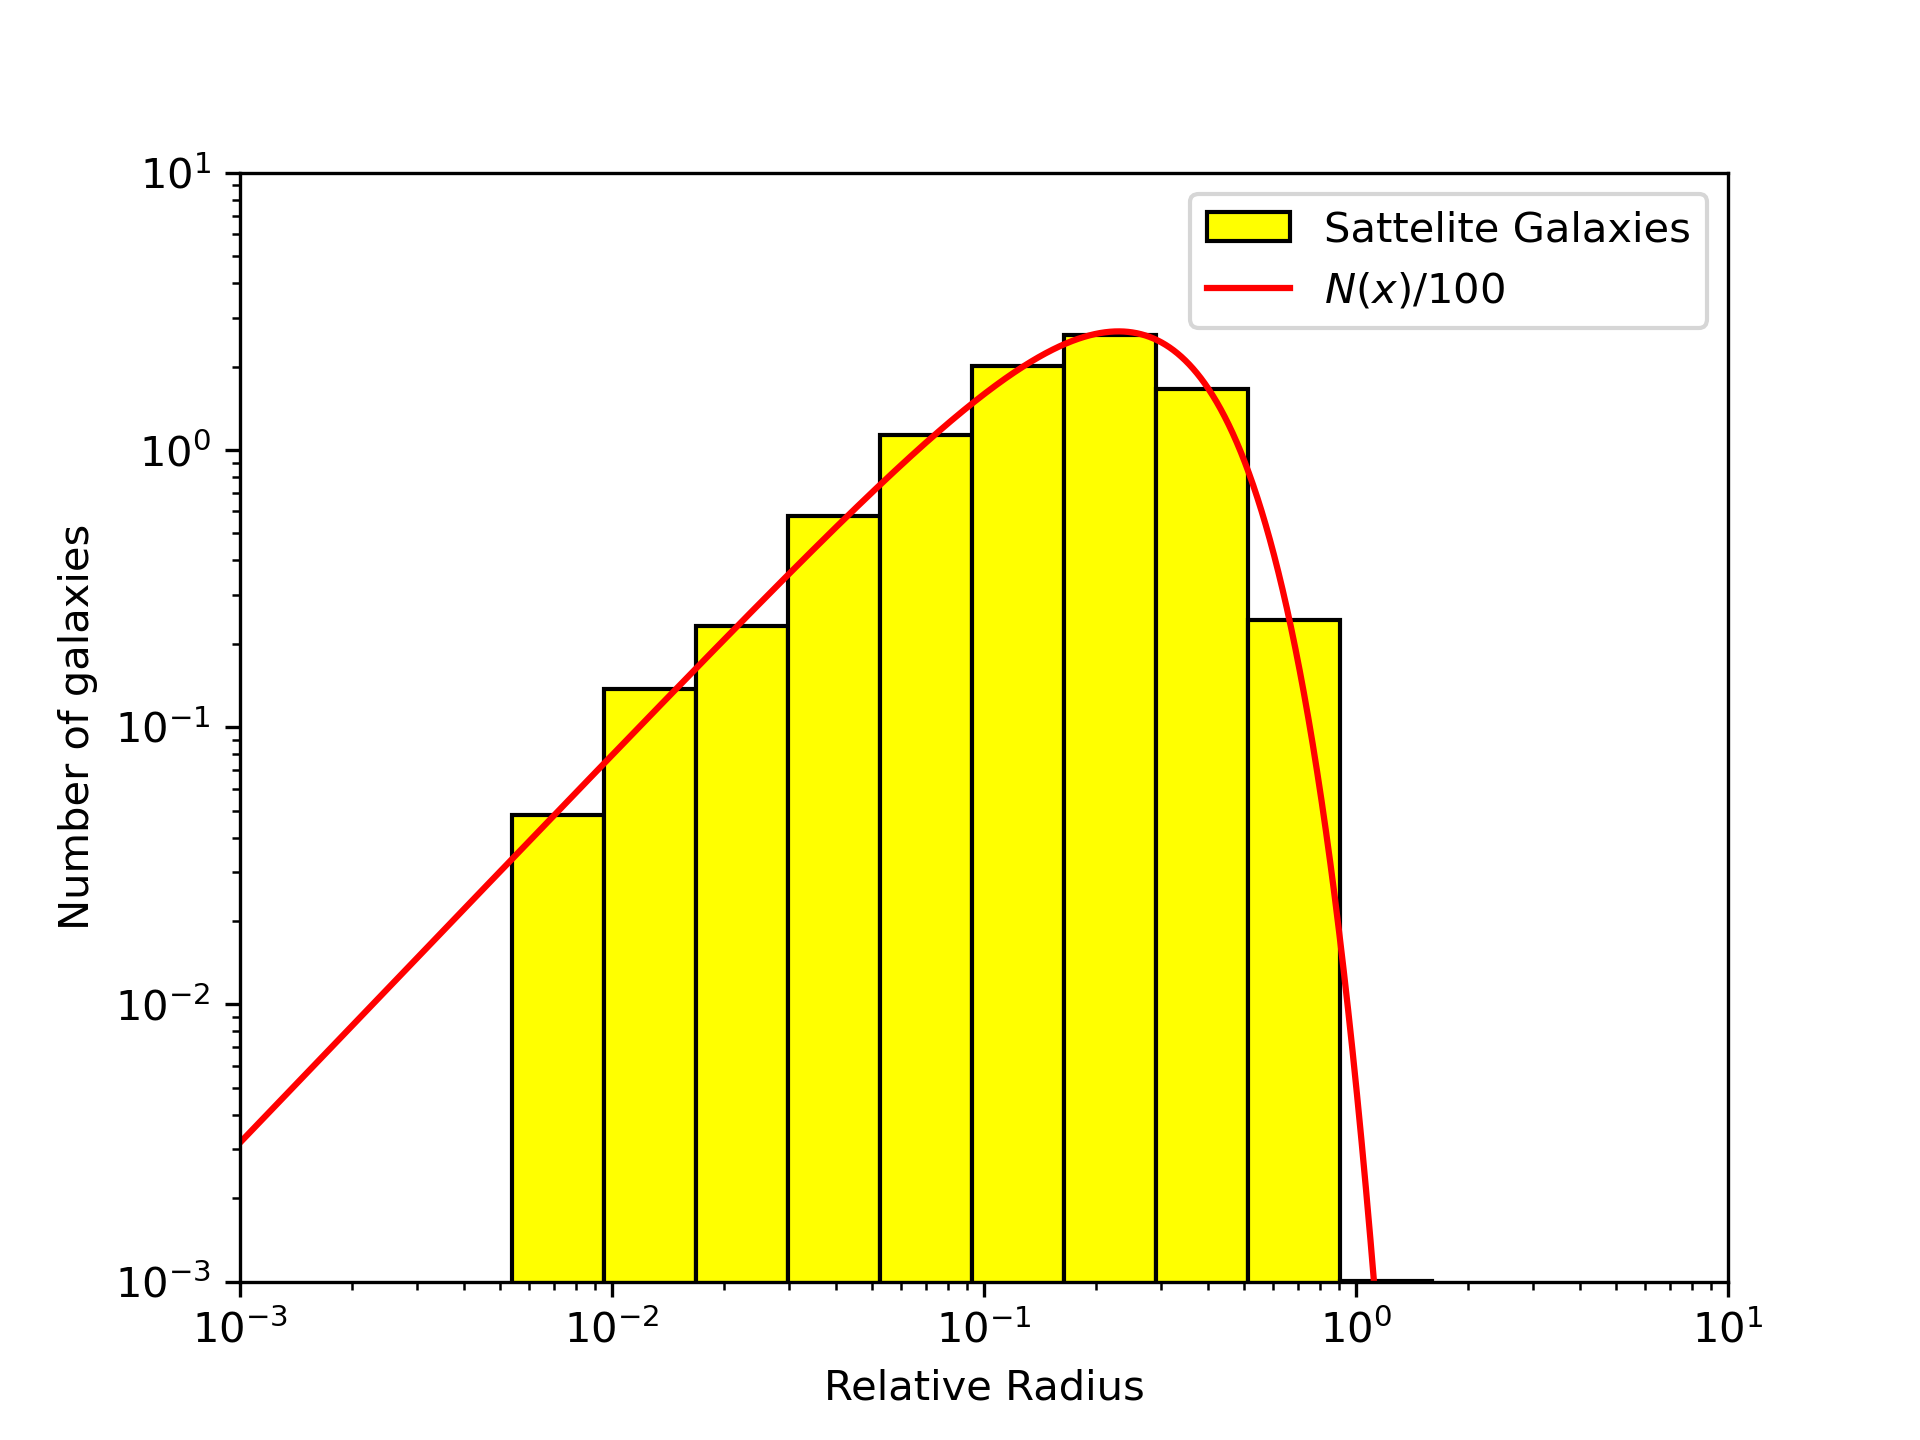
\includegraphics[width=0.49\linewidth]{./plots/distr_zoom.png}
  \caption{A histogram of the radii of the generated galaxies. Both the x and y axis, are in logarithmic scale. On the left panel, we can see the whole range that has a big empty space because the probability of the distribution is extremely low. On the right panel, we focus on the populated area of the distribution to see that our predictions match the given distribution.}
  \label{fig:distr}
\end{figure}

\subsection{Sorting 100 random galaxies}

We now want to select 100 galaxies from our sample. The process has to be random with every galaxy having an equal probability of being selected. We should have no duplicate galaxies in our selection and the process has to be done without rejecting any selection. We then want to sort the selected galaxies based on their relative radius and create a plot of galaxies within a radius.

To implement all that we first create a ``random\_selection'' function that uses the Fisher-Yates algorithm to completely randomize the array. We can then select the first N elements. This process follows all the principles we described, as every galaxy has an equal chance of getting selected, the elements are unique and we use no rejection. The Fisher-Yates algorithm works by utilizing our ``lcg'' generator. We first select N random numbers to be used as seeds. We then go through the array backwards and every time we generate a random integer in the range $[0,i]$. We then swap the elements. The final array is in random order. We can then choose the first N elements. 

To sort the selected galaxies we use the function ``selection\_sort'' that implements the known algorithm. Selection sort uses two loops. The second loop starts from the index of the first one, scans the unsorted part of the array to find the smallest element and then swaps it to the top of the sorted part of the array. When we finish the loops we will have an array that goes from the smallest to the biggest value.   

\lstinputlisting{sort.py}

\begin{figure}[H]
  \centering
  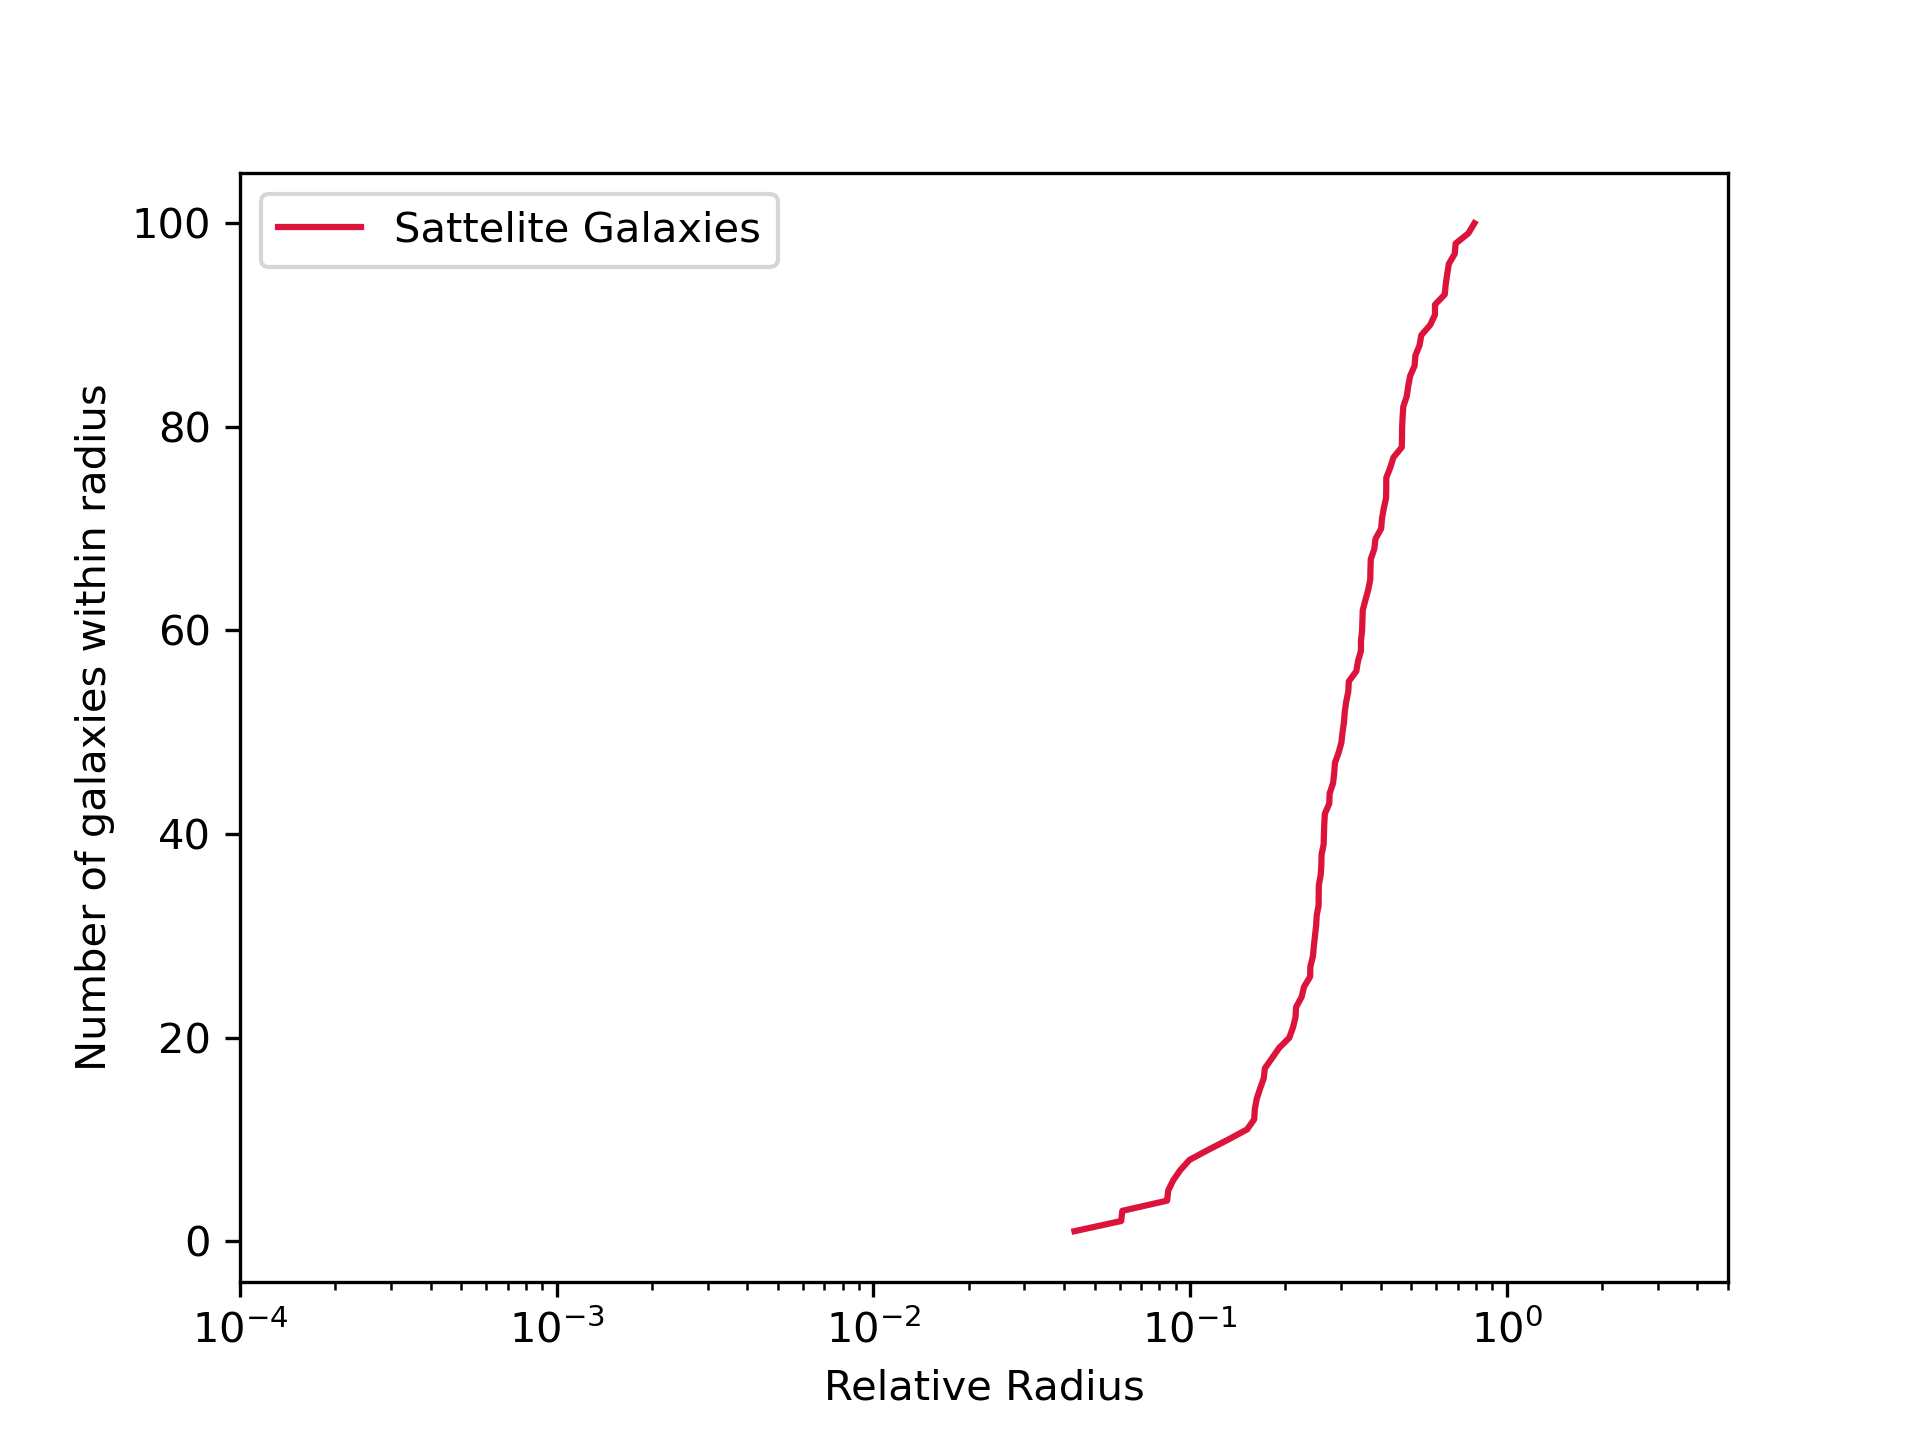
\includegraphics[width=0.6\linewidth]{./plots/rand_sort.png}
  \caption{The number of galaxies within a radius. We plot the 100 selected galaxies from our distribution and we plot how many galaxies we find within each value of the relative radius. The x-axis is in logarithmic scale.}
  \label{fig:sort}
\end{figure}

In the main part of our script, we load the sampled galaxies from our previous script. We then randomly select 100 elements which we then sort based on the value of the radius. We then want to plot the number of galaxies within a radius. We utilize the fact that we have the array sorted to use the values of radius as the x-values of our plot. For the y-values, we just need to increase by 1 every time a new element is found, which is done with the ``np.arange'' function. 

As we can see in \Cref{fig:sort} the sorting process worked at the plot is monotonically increasing within its range. 


\subsection{Numerical Differentiation}

In this part, we want to calculate the derivative of $n(x)$ at $x=1$. We aim for a precision of 12 significant digits or higher. To make sure of that we will compare our calculated value with the analytical solution of the derivative that we implemented in the function ``analyt\_der''. 

In our script, we import the function ``n'' with its parameters and also read the value of $A$ from the text file. The function ``f\_n'' acts as a wrapper, allowing us to define all the non-changing parameters. We then define the ``central\_dif'' function that calculates the derivative using the central difference algorithm. This function will be used inside the ``ridder'' function that uses Ridder's algorithm. The algorithm calculates the derivative multiple times using central differences for a decreasing step $h$ and then uses Richardson's extrapolation to combine the values. In our implementation the extrapolation stops when the estimated error increases, which allows us to give big values of $m$, knowing that it will not negatively affect our result.

\lstinputlisting{deriv.py}

In the main part of our script, we calculate the derivative using the ``ridder'' function. Notice that while we pass $m=10$, the function doesn't necessarily extrapolate to the 10th order as it can terminate before that if the estimated error increases. 

We also calculate the derivative by using the analytic function and print both with 14 significant digits. We also print the absolute difference between the two values.  

\lstinputlisting{output/deriv.txt}

As we can see the derivative we calculated matches the analytic one in all 14 significant digits. In fact, the absolute difference between the two values is $10^{-14}$. 

\section{Heating and cooling in HII regions}

In this section, we will numerically solve equations describing the process of heating and cooling HII regions. All the values and coefficients are given in c.g.s. units.

\subsection{First equation}

In our first approach, we only consider one heating and one cooling mechanism. The heating from photoionization can be described by:
\begin{equation}
  \Gamma_{pe}=\alpha_B n_H n_e \psi k_B T_c
\end{equation}
where $\alpha_B=2 \cdot 10^{-13}$ is the B recombination coefficient, $n_H$ and $n_e$ are the densities of hydrogens and electrons, $\psi=0.929$ is a numerical value, and $T_c=10^4$ is the stellar temperature.

The cooling mechanism in our scenario is by radiative recombination which follows the equation
\begin{equation}
  \Lambda_{rr}=\alpha_B n_H n_e \langle E_rr \rangle
\end{equation}
where 
\begin{equation}
  \langle E_rr \rangle = \left[0.684-0.0416 \ln\left(\frac{T}{10^4 Z^2}\right)\right]k_B T
\end{equation}

To find the equilibrium temperature we need
\begin{equation}
  \alpha_B n_H n_e \psi k_B T_c = \alpha_B n_H n_e \left[0.684-0.0416 \ln\left(\frac{T}{10^4 Z^2}\right)\right]k_B T
\end{equation}
or equivalently:
\begin{equation}
  \psi T_c - \left[0.684-0.0416 \ln\left(\frac{T}{10^4 Z^2}\right)\right] T = 0
\end{equation}

In our script, we define the equation we want to solve and use a wrapper to define all the values except the temperature. We then define two functions for root finding, ``false\_position'' and ``newton\_raphson''.

The false-position algorithm uses a bracket $[a,b]$ and calculates the new point at $c=\frac{a f_b-b f_a}{f_b-f_a}$. It then finds in which of the brackets $[a,c]$ or $[c,b]$ we have a change of sign to limit the original bracket. The process is repeated until we have a convergence to a predefined margin or the maximum number of iterations has been completed, in which case an error is raised. 

In the Newton-Raphson algorithm, we have a single value which is being updated, using the value of the derivative. To implement that we use the central difference algorithm from the previous task. The new point is calculated by: $a_{new} = a -\frac{f_a}{f'_as} $. 

The estimated error in both of these algorithms, which is being used to determine the convergence, is the relative error, which means that we divide it by the estimated true value. 

\lstinputlisting{root1.py}

We used both of our functions to numerically solve our equation. False-position worked in the general margin that was set by the problem $[1,10^7]$. In Newton-Raphson, we had to pick a starting point. When we chose the middle value $5\cdot 10^6$ the algorithm did not converge. When we instead used smaller initial values we had a fast convergence, much faster than when using the false-position. 

For each of the algorithms, the predefined accuracy that had to be reached for them to converge was set to $10^{-11}$. The final relative error estimates are even smaller as we can see in the output of the script. 

\lstinputlisting{output/root1.txt}


\subsection{Second equation}

We now want to add additional heating and cooling mechanisms and solve them. One such mechanism is the free-free emission cooling which is described by
\begin{equation}
  \Lambda_{FF}=0.54\left(\frac{T}{10^4}\right)^{0.37} \alpha_B n_H n_e k_B T
\end{equation}

The heating by cosmic rays can be calculated using
\begin{equation}
  \Gamma_{CR}=A n_e \xi_{CR}
\end{equation}
where $A=5\cdot 10^{-10}$ is a constant and $\xi_{CR}=10^{-15}$

One last heating mechanism comes from MHD waves 
\begin{equation}
  \Gamma_{MHD} = 8.9 \cdot 10^{-26} n_H \frac{T}{10^4}
\end{equation}

Combining all that and assuming $n_H=n_e$ (total ionization) we can derive an equation which can be solved numerically:
\begin{equation}
  (\psi T_c - \left[0.684-0.0416 \ln\left(\frac{T}{10^4 Z^2}\right)\right] T - 0.54\left(\frac{T}{10^4}\right)^{0.37}) k n_H \alpha_B + A \xi_{CR} + 8.9 \cdot 10^{-26} \frac{T}{10^4} = 0
\end{equation}

We will solve the above equation for three different values of $n_H=n_e$, which are $10^{-4}\, ,1\, , 10^4$. All values are again in c.g.s. units. 

For the root finding, we will use again the ``newton\_raphson'' algorithm from our previous script. We also define a new function ``secant'', which uses the secant algorithm for root finding. In this algorithm, we have two initial points (that can act as a bracket). The new point is calculated using: $c=b-f_b\frac{b-a}{f_b-f_a}$. We then set $a=b$ and $b=c$ and repeat the process until the relative difference between the two values reaches the desired accuracy. 

\lstinputlisting{root2.py}

In the main part of our script, we find the roots for the different values of $n_H$ using both algorithms. The secant algorithm did not converge for $n_H=10^{-4}$. For the other two values of $n_H$, it managed to find the correct value of the temperature in the least number of iterations (9 and 8). All the equations were solved in the range $[1,10^{15}]$ 

The Newton-Raphson algorithm managed to solve the equation for all values of $n_H$. The number of iterations needed was 22 for the two higher values of $n_H$, while for the smallest density, it only needed 9 iterations. Note that in this method we use only one starting point which we set at the middle of our range ($5 \cdot 10^{14}$) 

For all these implementations we stopped when the relative accuracy reached was below $10^{-11}$. As we can see in the output they achieved relative accuracies ranging from $10^{-13}$ to $10^{-17}$

\lstinputlisting{output/root2.txt}

Lastly, one thing that becomes clear from the values of the temperature for the equilibrium, is that it greatly depends on the density of the hydrogen (which is equal to the electron). The low-density gas had a much higher temperature of equilibrium ($10^{14}$) when compared with the higher-density ones ($10^{4}$).

\subsection{Timing executions}

In this last part, we want to time the functions we used to solve the previous equations. For each one, we select the implementation that used the least number of iterations and we time it for $10^5$ executions and take the average time. 

For equation 1 we calculated the average time using the ``false\_position'' and the ``newton\_raphson''. For the 2nd equation, we calculate the average time using the ``newton\_raphson'' for $n_H=10^{-4}$ and the ``secant'' for the other two values of the density. 

\lstinputlisting{time_2.py}

We can see that for all the implementations the average time is at the order of $10^{-5}\: s$. Newton-Raphson is the fastest for equation 1 (it also used the least number of iterations), while for the different density values of equation 2, the secant algorithm is the fastest when it is able to converge, which is not the case for the low density. For this case, the best we can do is use Newton-Raphson which is relatively slower. 

\lstinputlisting{output/time_2.txt}

\end{document}
